\section{Figures}

\textbf{Figure 1.} Schematics of the analysis setup. Different parts of
the analysis were done in different software environments (see text).
Analysis feature layers (index layers) were constructed from 3 different
data sources (Table 1 and a condition layer (see text) was applied on
all of them. Different Zonation analysis variants are indicated by
arrows 1-4 (see Table 3) with closed circles indicating the analysis
features used. Each analysis variant resulted in a priority maps (Figure
2) and feature-specific performance curves (Figure 3). For validation
purposes, each rank priority map was compared to a set of independent
validation data to determine the mean and the distribution of ranks
(Figure 4).

\textbf{Figure 2.}

\begin{figure}
  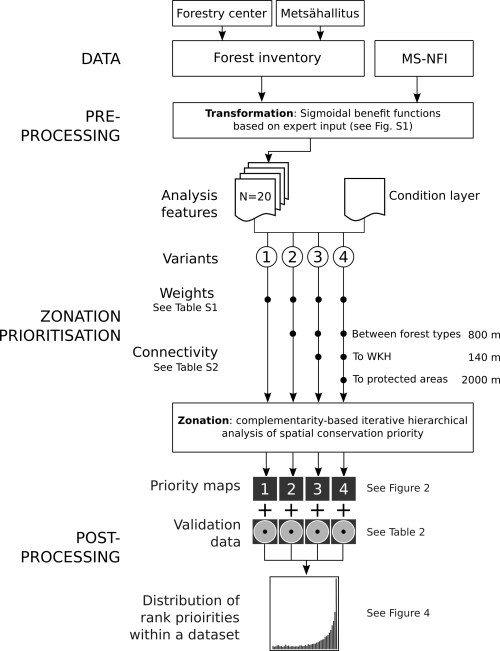
\includegraphics{figs/Fig1_w500.png}
  \caption{Schematics of the analysis setup.}
  \end{figure}

\begin{figure}[htbp]
\centering
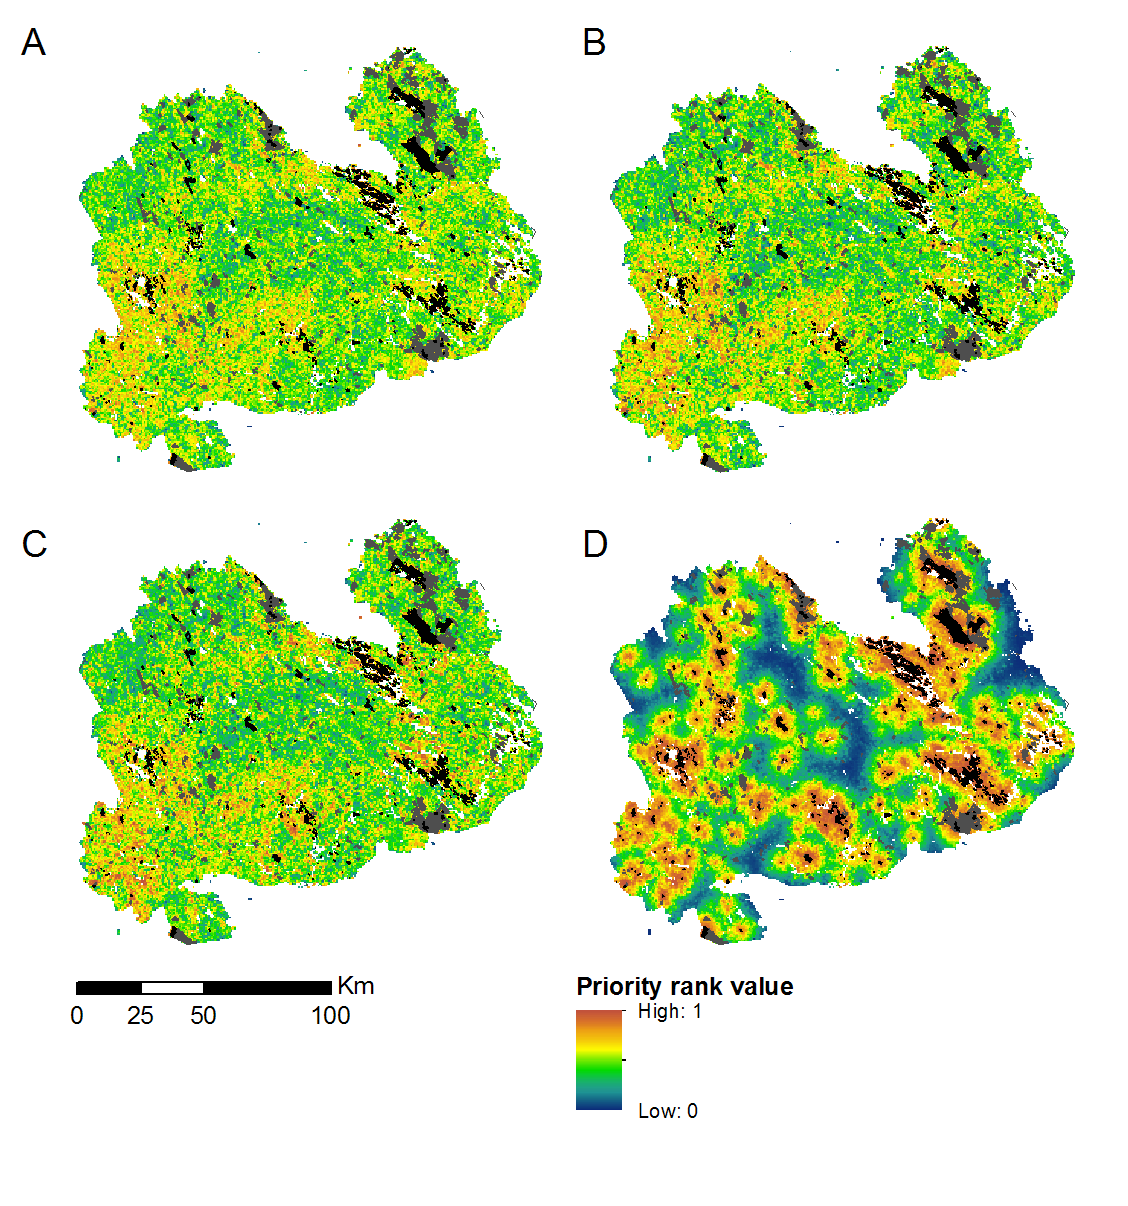
\includegraphics{figs/Fig2.png}
\caption{Figure2}
\end{figure}

\begin{figure}[htbp]
\centering
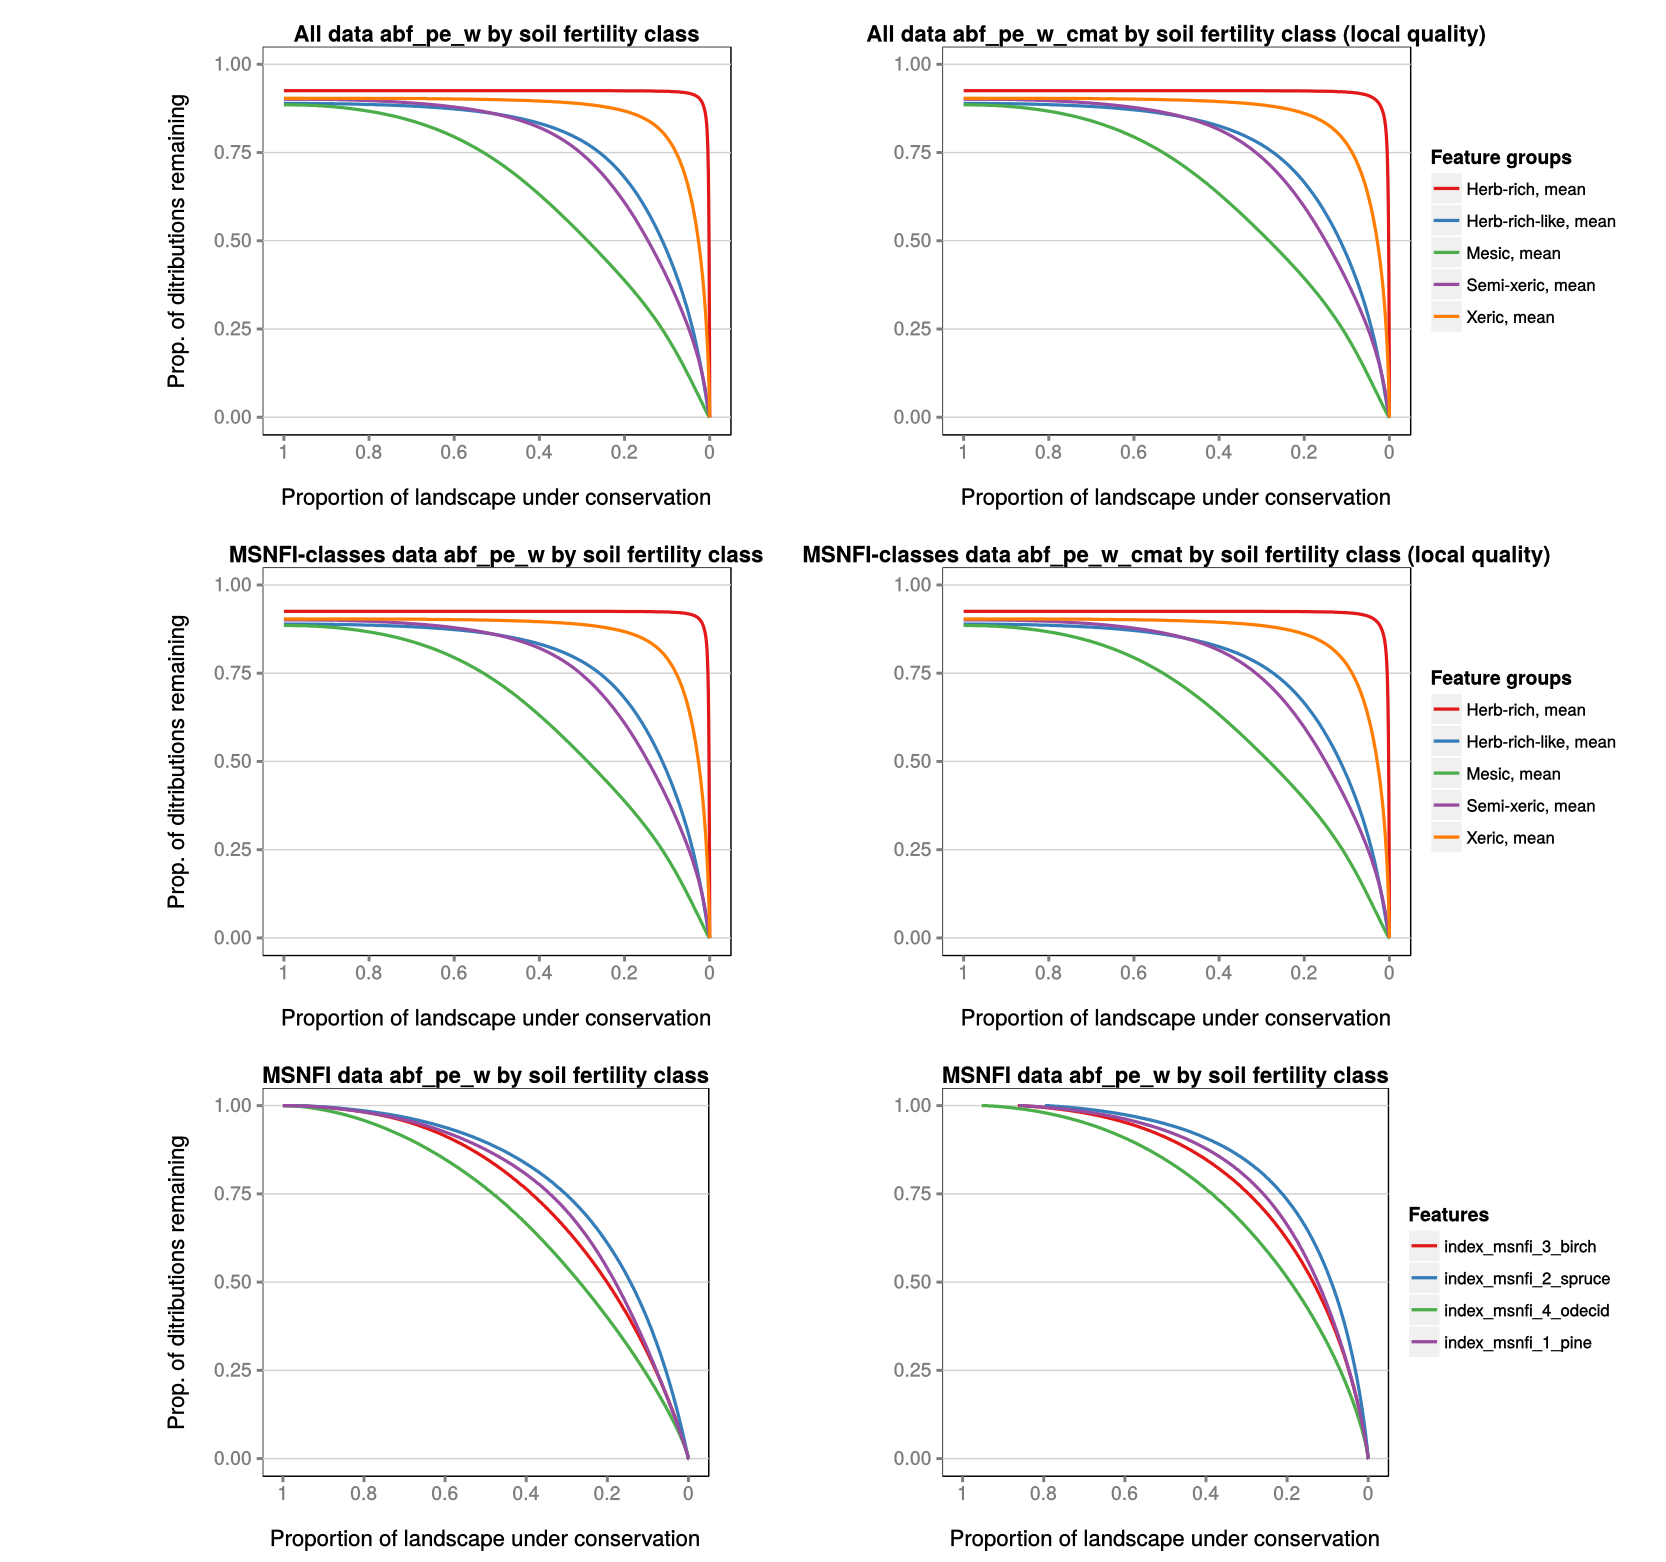
\includegraphics{figs/Fig3.png}
\caption{Figure3}
\end{figure}
